\section{Introducci\'on}

\subsection{Información}

\par La \textbf{información} de un evento aleatorio $e$ con probabilidad $P(e)$ está dada por:

\begin{equation*}
    I(e) := -log_b(P(e))
\end{equation*}

para una cierta base $b$. 
La elección de dicha base determina la unidad de la información; en este trabajo nos limitaremos a base 2, por lo que la unidad que manejaremos son los \textit{bits}. 

\par La \textbf{entropía} de una variable aleatoria $A$ es la esperanza de la información de $A$, y está dada por:

\begin{equation*}
    H(A) := \sum_{a \in A}{P(a) * I(a)} = - \sum_{a \in A}{P(a) * log(P(a))}
\end{equation*}

\par La entropía máxima de una variable aleatoria se da cuando los eventos son equiprobables.
En particular, para una variable Bernoulli\footnote{Es decir, una que admite sólo dos eventos posibles.} equiprobable, la máxima entropía es de 1 bit.

\par Una \textbf{fuente} emite mensajes con ciertas probabilidades.
Una \textbf{fuente de memoria nula} es una en la cual la probabilidad de cada mensaje no depende de los mensajes previos; viendo cada mensaje como una variable aleatoria, esto equivale a que sean independientes.
Adicionalmente, si la probabilidad de cada mensaje es constante en el tiempo\footnote{A partir de ahora, asumiremos que lo es.}, estas variables además son idénticamente distribuidas.

\par La entropía de una fuente de memoria nula es la entropía de cada mensaje, que equivale a la información esperada de cada mensaje.

\subsection{Capa de enlace y ARP}

\par En la mayoría de los protocolos de la capa de enlace se emplean identificadores únicos; en el caso de Ethernet (802.3) y WLAN (802.11), este identificador lleva el nombre de MAC (\textit{Media Access Control}) address.

\par Un frame de una red Ethernet puede ser transmitido de forma \textit{unicast}, es decir para sólo un receptor\footnote{Debido a la naturaleza de Ethernet, se transmite a toda la red, pero los otros receptores normalmente descartarán los frames que no les son destinados.}, especificando como destino su MAC address; o de forma \textit{broadcast}, es decir para todos los dispositivos de la red, marcando como desinto la MAC address FF:FF:FF:FF:FF:FF.

\par Generalmente, la transmisión \textit{broadcast} se emplea para protocolos de control (por ejemplo ARP o detección de colisiones en Ethernet), mientras que la \textit{unicast} podrá enviar datos\footnote{También podrá ser utilizada por algunos protocolos de control, por ejemplo ARP, como se detallará a continuación.}.

\par También es ubicuo el uso de los identificadores únicos en la capa de red; para el protocolo más común (IP), se utilizan Direcciones IP.

\par Para relacionar un identificador de capa de red con uno de capa de enlace\footnote{En nuestro caso, Direcciones IP y MAC addresses, respecitvamente. De aquí en adelante utilizaremos estos términos al referirnos a ARP.}, se emplea el protocolo ARP (\textit{Address Resolution Protocol}).
En la figura \ref{ARPpacket} se puede ver la estructura de un paquete ARP.

\begin{figure*}[ht]
    \centering
    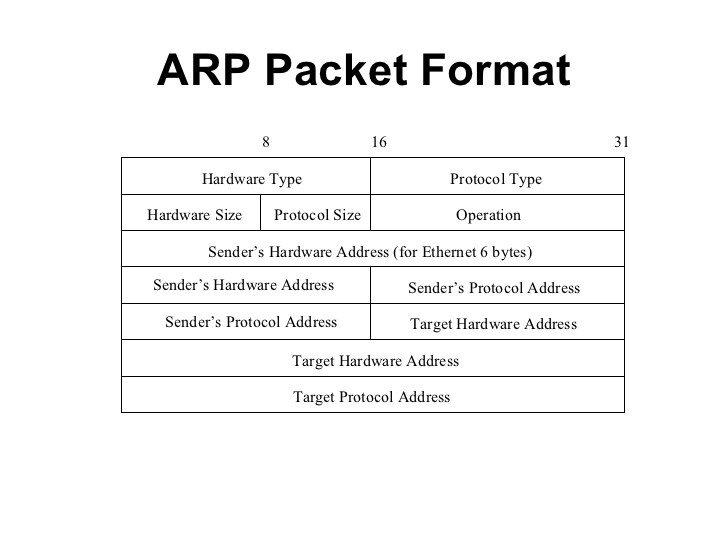
\includegraphics[width=0.9\textwidth]{figuras/ARPpacket}
    \caption{Estructura de un paquete ARP.}\label{ARPpacket}
\end{figure*}

\par Para encontrar la MAC address correspondiente a una Dirección IP conocida, un dispositivo envía un paquete a la red de forma \textit{broadcast}.
Marca en 1 el campo Operation (\textit{who-has}), anota su Dirección IP y su MAC address en los campos \textit{Sender's Protocol Address} y \textit{Sender's Hardware Address}, respectivamente, y escribe la Dirección IP deseada en el field \textit{Target Protocol Address}.

\par Cuando un dispositivo recibe el paquete e identifica a su propia Dirección IP como la \textit{Target Protocol Address}, responde enviando otro paquete ARP al emisor original.
En este caso, el campo Operation se settea en 2 (\textit{is-at}).
Ambos campos de \textit{Sender's Address} nuevamente se completan con sus direcciones, mientras que los de \textit{Target Address}, con las direcciones provistas por el emisor en el paquete \textit{who-has} original.

\par Cabe destacar que un paquete \textit{who-has} debe ser enviado de forma \textit{broadcast} (ya que la MAC address del receptor es desconocida), mientras que uno \textit{is-at} se transmite de forma \textit{unicast}, pues el emisor original envió su MAC address en el request original.

\par Adicionalmente, hay dos casos de uso especiales de ARP: \textit{ARP probing} y \textit{gratuitous ARP}.
El primero se emplea para evitar colisiones en los identificadores de IP (específicamente en IPv4, la versión más común actualmente), y se destaca al señalar el campo \textit{Sender's Protocol Address} con todos 0\footnote{El valor específico es 0.0.0.0.}.
El segundo se usa como anuncio, y en éste se marcan los campos de \textit{Sender's Protocol Address} y \textit{Target Protocol Address} con la dirección IP del dispositivo que realiza el anuncio. 
